\section{An interval-pair inequality}\label{sec:intervals}

We first isolate the geometric comparison used in the pressure estimate.
It is a statement about two parallel lines and does not involve the
equations. The self-contained midpoint argument below gives the
comparison; its nonnegative formulation also permits unbounded
intervals of weight zero.

Fix a unit vector $e$ and distinct $z,z'\in e^\perp$.  Write
\[
 x=z+se,\qquad y=z'+s'e,\qquad
 \lambda=|z-z'|>0,\qquad h=s-s'.
\]
The restricted Newton kernel and its directional factor are
\[
 \mathcal K(s,s')
 =\frac{(\lambda^2+h^2)^{(2-n)/2}}{(n-2)|\Sph|},
 \qquad \mathcal D(s,s')=\frac{h^2}{\lambda^2+h^2}.
\]
For a bounded interval $I=(s_-,s_+)$, let
\[
 \overline{\mathcal K}_I(s')
 =\frac{\mathcal K(s_-,s')+\mathcal K(s_+,s')}{2}.
\]
For a bounded interval $J=(s'_-,s'_+)$, define
$\overline{\mathcal K}_J(s)$ by averaging in the second variable.
When $I$ and $J$ are bounded, write $m_I,m_J$ for their midpoints and
$d_0=m_I-m_J$ for their midpoint separation.

\begin{figure}[htbp]
\centering
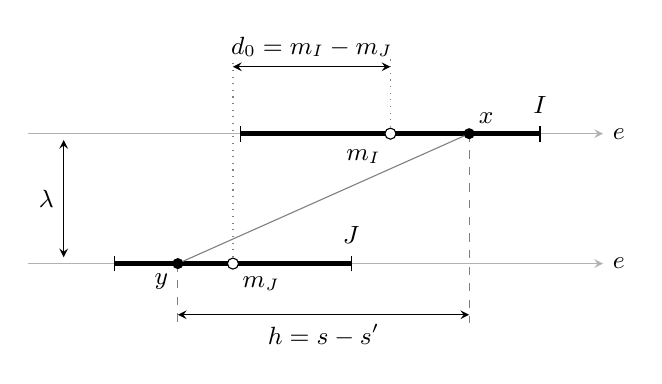
\begin{tikzpicture}[x=1cm,y=1cm,>=stealth, font=\small]
 \draw[gray!60,->] (-0.3,1.65)--(7,1.65);
 \draw[gray!60,->] (-0.3,0)--(7,0);
 \draw[line width=1.6pt] (2.4,1.65)--(6.2,1.65);
 \draw[line width=1.6pt] (0.8,0)--(3.8,0);
 \draw (2.4,1.55)--(2.4,1.75) (6.2,1.55)--(6.2,1.75);
 \draw (0.8,-0.1)--(0.8,0.1) (3.8,-0.1)--(3.8,0.1);
 \node[above] at (6.2,1.78) {$I$};
 \node[above] at (3.8,0.13) {$J$};
 \node[right] at (7,1.65) {$e$};
 \node[right] at (7,0) {$e$};
 \draw[<->] (0.15,0.08)--node[left] {$\lambda$}(0.15,1.57);
 \draw[gray,dashed] (1.6,0)--(1.6,-0.75);
 \draw[gray,dashed] (5.3,1.65)--(5.3,-0.75);
 \draw[<->] (1.6,-0.65)--node[below] {$h=s-s'$}(5.3,-0.65);
 \draw[gray] (1.6,0)--(5.3,1.65);
 \fill (5.3,1.65) circle (2pt);
 \fill (1.6,0) circle (2pt);
 \node[above right] at (5.3,1.65) {$x$};
 \node[below left] at (1.6,0) {$y$};
 \draw[gray,dotted] (2.3,0)--(2.3,2.6);
 \draw[gray,dotted] (4.3,1.65)--(4.3,2.6);
 \draw[<->] (2.3,2.5)--node[above] {$d_0=m_I-m_J$}(4.3,2.5);
 \fill[white] (4.3,1.65) circle (2pt);
 \draw (4.3,1.65) circle (2pt);
 \fill[white] (2.3,0) circle (2pt);
 \draw (2.3,0) circle (2pt);
 \node[below left] at (4.3,1.57) {$m_I$};
 \node[below right] at (2.3,-0.04) {$m_J$};
\end{tikzpicture}
\caption{The transverse separation is $\lambda$, whereas the kernel
depends on the longitudinal difference $h$.  The distribution of $h$
over $I\times J$ is symmetric about the midpoint separation $d_0$,
which need not be zero.}
\label{fig:interval-geometry}
\end{figure}

\begin{lemma}[Weighted interval comparison]\label{lem:interval-pair}
Let $n\ge3$, $\lambda>0$, and let $I,J\subset\R$ be nonempty open
intervals, possibly unbounded.  Let $c_I,c_J\ge0$, with $I$ bounded
whenever $c_I>0$ and $J$ bounded whenever $c_J>0$.  Then
\begin{equation}\label{eq:interval-pair}
\begin{split}
 \int_{I\times J}(c_I+c_J)\mathcal K\,\dd s\,\dd s'
 \le \int_{I\times J}\Bigl[
 &c_I\overline{\mathcal K}_I+c_J\overline{\mathcal K}_J\\
 &+\bigl((n-2)\min(c_I,c_J)\mathcal D
                  +|c_I-c_J|\bigr)\mathcal K\Bigr]\,\dd s\,\dd s'.
\end{split}
\end{equation}
Every term is nonnegative and the inequality is understood for extended
integrals.  An endpoint term with coefficient zero is defined to be zero,
without evaluating the endpoint average.
\end{lemma}

\begin{proof}
If at most one coefficient is positive, then
$|c_I-c_J|=c_I+c_J$, so the inequality holds pointwise before integration.
Suppose now that both coefficients are positive.  Both intervals are
bounded and $\lambda>0$, so all integrals in the following calculation
are finite.

Integration by parts in the first variable gives
\[
 \int_I(\mathcal K-\overline{\mathcal K}_I)\,\dd s
 =-\int_I(s-m_I)\partial_s\mathcal K\,\dd s.
\]
The corresponding identity in the second variable, together with
\[
 \partial_s\mathcal K=-(n-2)\frac{h}{\lambda^2+h^2}\mathcal K,
 \qquad
 \partial_{s'}\mathcal K=(n-2)\frac{h}{\lambda^2+h^2}\mathcal K,
\]
yields
\begin{equation}\label{eq:midpoint-identity}
 \int_{I\times J}
  (2\mathcal K-\overline{\mathcal K}_I-\overline{\mathcal K}_J)
   \,\dd s\,\dd s'
 =(n-2)\int_{I\times J}
    \frac{h^2-d_0h}{\lambda^2+h^2}\mathcal K\,\dd s\,\dd s'.
\end{equation}

The sign of the midpoint term follows directly from interval overlap.
If $L=|I|$ and $M=|J|$, the pushforward of $\dd s\,\dd s'$ under
$(s,s')\mapsto h=s-s'$ has density
\[
 \rho(h)=F(|h-d_0|),\qquad
 F(r)=\max\left\{0,\min\left\{L,M,\frac{L+M}{2}-r\right\}\right\}
 \quad(r\ge0).
\]
Indeed, $\rho(h)=|I\cap(J+h)|$, the overlap length of two intervals
whose centers are separated by $|h-d_0|$.
The function $F$ is nonincreasing.  If $d_0\ge0$ and $h>0$, then
$|h-d_0|\le|h+d_0|$, hence $\rho(h)\ge\rho(-h)$; for $d_0\le0$
the inequality is reversed.  Pairing positive and negative $h$ against
the odd function
$h\mathcal K(h)/(\lambda^2+h^2)$ therefore proves
\[
 d_0\int_{I\times J}\frac{h}{\lambda^2+h^2}
                 \mathcal K\,\dd s\,\dd s'\ge0.
\]
Consequently the left side of \eqref{eq:midpoint-identity} is at most
$(n-2)\int_{I\times J}\mathcal D\mathcal K$.

Multiply this last estimate by $c=\min(c_I,c_J)$.  Each individual
endpoint defect is bounded above by $\int_{I\times J}\mathcal K$,
because its subtracted endpoint average is nonnegative.  The remaining
coefficients are $c_I-c$ and $c_J-c$, whose sum is $|c_I-c_J|$.
Adding these estimates and moving the finite endpoint terms to the
right proves \eqref{eq:interval-pair}.
\end{proof}

The nonnegative formulation is essential when $n=3$: even for
$\lambda>0$, an integral of $\mathcal K$ over an unbounded partner
interval can diverge.  Lemma~\ref{lem:interval-pair} makes no subtraction
on such an interval.
